\section{Zu Beginn \dots}

\begin{frame}
\begin{block}{Kurze Vorstellungsrunde}
	\vspace{2pt}
	Schaffst Du es \emph{in 60 Sekunden} folgende Fragen möglichst knackig und aussagekräftig zu beantworten?
	\begin{itemize}
		\item Wer bist Du? 
		\item Windows, Mac oder Linux?
		\item Welche Vorkenntnisse hast Du beim Programmieren?  
		\item Warum hast Du Dich zum Python-Kurs angemeldet? 
		\item Wann wäre der Kurs für Dich perfekt gelaufen? (Best Case Szenario)
		\item Wann würdest Du den Kurs nicht weiter besuchen? (Worst Case Szenario)
	\end{itemize}
\end{block}
\end{frame}


\begin{frame}
	\begin{block}{Ablauf des Kurses}
		\begin{itemize}
			\item Mischung aus Vortrag, Live-Coding und Präsenzübungen
			\item Im Idealfall: Mehr Praxis statt Erklärungen
			\item Jede Woche gibt's ein Aufgabenblatt $\rightarrow$ Besprechung in der nächsten Woche
			\item Kommunikation über Slack: \texttt{https://bit.ly/3a5W9fE} 
			%\texttt{python-kurs.slack.com} 
			(freiwillig)
		\end{itemize}
	\end{block}
\end{frame}

\begin{frame}
	\begin{block}{Warum Python?}
		\begin{itemize}
			\item Einfaches Setup
			\item Einstiegsfreundliche Syntax
			\item Python ist eine Hochsprache
			\item Python muss nicht kompiliert, sondern nur interpretiert werden
			\item Große Community $\rightarrow$ großes \emph{Ecosystem}
			\item Python ist extrem vielseitig
			\item Python ist plattformunabhängig
		\end{itemize}
	\end{block}
\end{frame}

\begin{frame}
	\begin{block}{Typische Einsatzbereiche}
		\begin{itemize}
			\item Automatisierung
			\item Webscraping
			\item Datenanalyse
			\item Webentwicklung
		\end{itemize}
	\end{block}
\end{frame}

\begin{frame}
\begin{block}{Phasen des Lernens einer Programmiersprache}
	\vspace{2pt}
	\uncover<+->{
\begin{enumerate}[<+->]
	\item Annäherung:  Fokus auf dem Begreifen der Grundkonzepte
	\item Syntax: Fokus auf der korrekten Anwendung der Syntax
	\item Funktionalität: Fokus liegt darauf, Problemstellungen \emph{pragmatisch} zu lösen
	\item Design: Fokus auf les-und wartbaren Code
	\item Architektur: Fokus auf Strategie, Projekte nachhaltig und erweiterbar umzusetzen 
\end{enumerate}
	}
\end{block}
\end{frame}


\begin{frame}
	\metroset{block=fill}
	\uncover<+->{\begin{block}{Was wird benötigt?}
			\vspace{2pt}
			\uncover<+->{
				\textbf{Am Anfang}
				\begin{itemize}
					\item Compiler/Interpreter
					\item Texteditor (z.B. Mac: Xcode, Windows: Edit)
				\end{itemize}
			}
			\uncover<+->{
				\textbf{Später}
				\begin{itemize}
					\item Google
					\item Integrierte Entwicklungsumgebung (IDE)
					\item Versionskontrolle (VCS)
					\item Virtueller Maschinen
					\item Datenbanken
					\item Grafikbearbeitung
				\end{itemize}
			}
	\end{block}}
\end{frame}

\begin{frame}
\begin{block}{Wo findet man Hilfe/Infos?}
	\vspace{2pt}
	\begin{itemize}
		\item Google
		\item \texttt{stackoverflow.com}
		\item Youtube (z.B. Tutorials)
		\item Austausch über Slack 
		\item \texttt{docs.python.org/3}
		\item Bücher (z.B. \textit{Python Crashkurs} v. \textsc{Eric Matthes})
		\item \texttt{mailto: aaron.kunert@salemkolleg.de}
	\end{itemize}
\end{block}
\end{frame}


\section{Installation von Python}

\begin{frame}
\begin{block}{Ist Python schon installiert ?}
	\begin{itemize}
		\item Öffne ein Terminal/die Eingabeaufforderung
		\item Gib ein \bash{python --version}
		\item oder alternativ \bash{python3 --version}
		\item Erhältst Du die Antwort \bash{Python} und eine Zahl $\geq 3.6$, dann ist alles fein
		\item Falls nicht: Installiere Python!
	\end{itemize}
\end{block}
\end{frame}


\begin{frame}
\begin{block}{Installation}
\begin{enumerate}
	\item Gehe auf https://www.python.org/downloads/
	\item Klicke den Button "Download Python 3.9.3."
	\item Führe die Installationsdatei aus
	\item Falls Du gefragt wirst, bestätige, dass Python zum PATH hinzugefügt wird
	\item Eventuell muss der Rechner neu gestartet werden
\end{enumerate}	
\end{block}

\begin{alertblock}{Achtung bei Windows}
\vspace{2pt}
Python muss zum PATH hinzugefügt werden. 

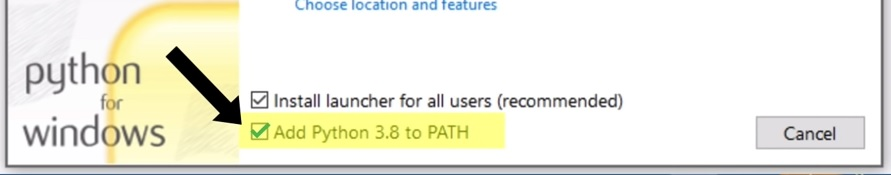
\includegraphics[width=0.65\textwidth]{python_path.jpg}
\end{alertblock}

\end{frame}

\begin{frame}
\begin{block}{Cross-Check}
\vspace{2pt}
Gib \bash{python} (Win) oder \bash{python3} (Mac) im \textit{Terminal} ein.
Du solltest etwa folgendes sehen:  
\vspace{12pt}

\texttt{Python 3.9.2 (tags/v3.9.2:1a79785, Feb 19 2021, 13:44:55) [MSC v.1928 64 bit (AMD64)] on win32
	Type "help", "copyright", "credits"{} or "license"{} for more information.}

\texttt{>{}>{}>}
\end{block}
\begin{block}{}
Jetzt bist Du im \textit{interactive mode} (REPL) von Python. Hier kannst Du einzelne Codezeilen eingeben und mittels \bash{Enter} ausführen. 
Um den interactive mode zu verlassen, gib \py{exit()} ein und bestätige mit der \bash{Enter}-Taste. 	
\end{block}
\end{frame}


%\begin{standout}
%	Erste Schritte im Interactive Mode\\
%\end{standout}
\section{Erste Schritte im REPL \\ \footnotesize (Read-Evaluate-Print-Loop)}


\begin{frame}
\begin{block}{Probier mal folgende Kommandos aus}	
	\begin{itemize}
		\item \py{3 + 4}
		\item \py{2 - 7}
		\item \py{"Hello" + "Python"}
	\end{itemize}
\end{block}	
\end{frame}



\begin{frame}{Übung}
\uncover<+->{\begin{block}{Was machen die folgenden \textit{Operatoren}?}
	\begin{itemize}
		\item \pybw{+}
		\item \pybw{-}
		\item \pybw{*}
		\item \pybw{/}
		\item \pybw{**}
	\end{itemize}
\end{block}}
\uncover<+->{\begin{block}{Und diese?}
\begin{itemize}
		\item \%
		\item \pybw{//}
		\item \pybw{==}
		\item \pybw{<=}
		\item \pybw{<}
\end{itemize}
\end{block}}

\end{frame}

\begin{frame}{Übung}
	\begin{block}{Wie rechnet Python?}
		\begin{itemize}
			\item Wird Punkt-vor-Strich berücksichtigt?
			\item Kann man mit Klammern die Reihenfolge beeinflussen?
			\item Was ist der Unterschied zwischen \py{10/5} und \py{10//5} ?
			\item Was bedeutet das Kommando \py{_}? 
			\item Wie kann man Zwischenergebnisse in Variablen speichern?
		\end{itemize}
	\end{block}
\end{frame}

\section{Variablen}

\begin{frame}
\uncover<+->{\begin{block}{}
		Jeder Wert in Python kann in einer Variable gespeichert werden: 
		
		\py{my_variable = 3}
\end{block}}

\uncover<+->{\begin{block}{}
		Die Zuweisung darf auch das Ergebnis einer Berechnung sein: 
		
		\py{my_new_variable = 3 + 5}
\end{block}}
\uncover<+->{\begin{block}{}
		Die Zuweisung darf auch weitere Variablen enthalten: 
		
		\py{my_brand_new_variable = my_variable + my_new_variable }
\end{block}}

\uncover<+->{\begin{block}{}
	Man darf auch Kettenzuweisungen machen: 
	
	\py{a = b = c = 100 }
\end{block}}
\end{frame}


\begin{frame}
\uncover<+->{\begin{block}{Gültige Variablennamen}
\begin{itemize}[<+->]
	\item Erlaubt sind Buchstaben (nur ASCII), Ziffern und Unterstriche
	\item Der Name darf nicht mit einer Ziffer starten
	\item Beliebige Länge 
	\item Wer's schon kennt als \emph{regulärer Ausdruck}:  \mintinline{php}{[_a-zA-Z][_0-9a-zA-Z]*}
	\item Schlüsselwörter sind nicht erlaubt
\end{itemize} 
\end{block}}
\vspace{12pt}
\uncover<+->{\begin{block}{Liste der Schlüsselwörter}
	\texttt{
	\begin{columns}[T,onlytextwidth]
		\column{0.2\textwidth}
		False\\ 	await\\ 	else\\ 	import\\ 	pass\\ assert \\	del\\ 	
		\column{0.2\textwidth}
		None \\	break \\	except \\ 	in \\	raise \\ global \\	not \\	 
		\column{0.2\textwidth}
		True \\	class \\ 	finally \\ 	is \\	return \\ with \\ async 
		\column{0.2\textwidth}
		and \\	continue \\ 	for \\	lambda \\	try \\ 	elif  \\	if  \\
		\column{0.2\textwidth}
		as \\ 	def \\ 	from  \\	nonlocal \\	while \\ 	or \\ 	yield
	\end{columns}
}
\end{block}}
\end{frame}


\begin{frame}
\uncover<+->{\begin{exampleblock}{Style-Guide Variablennamen}
	\begin{itemize}
		\item Englische Wörter
		\item Nur Kleinbuchstaben
		\item Möglichst aussdrucksstarke Namen verwenden
		\item Keine Angst vor langen Namen 
		\item Namen, die aus mehreren Worten bestehen, mit Unterstrich trennen (\textit{snake-case})
	\end{itemize}
	
	\uncover<+->{z.B. \py{students_in_this_room}, \py{number_of_unpaid_bills}}
\end{exampleblock}}

\end{frame}

\begin{frame}{Übung}
	
	\begin{block}{Probier's aus!}
		\begin{itemize}
			\item Welchen Wert hat eine Variable, wenn man sie nicht vorher definiert hat? 
			\item Was passiert, wenn man eine Variable definiert, die schonmal verwendet wurde?
			\item Wie kann man eine Variable mit Wert \py{3} um \py{1} vergrößern?
		\end{itemize}	
	\end{block}
	
\end{frame}


\section{Datentypen}

\begin{frame}
	\begin{block}{}
		Jeder Wert in Python hat einen \textit{Datentyp}. Unter anderem gibt es folgende \textit{primitive} Typen in Python.
		\begin{itemize}
			\item \py{int}  Integer (ganze Zahlen)
			\item \py{float} Float (Dezimalzahlen)
			\item \py{bool} Boolean (Wahrheitswerte)
			\item \py{str}  String (Zeichenketten)
			\item \pybw{NoneType} (Typ des leeren Werts \py{None})
		\end{itemize}
	\end{block}
\end{frame}


\begin{frame}
	\metroset{block=fill}
	
	\uncover<+->{\begin{block}{Integer}
		Ganze Zahlen wie z.B. \py{1}, \py{-1}, \py{0}. Nicht aber 
		\py{2.0} oder \py{0.0}. 	
	\end{block}}
	\vspace{12pt}
	\uncover<+->{\begin{block}{Float}
		Fließkommazahlen, z.B. \py{3.1415925}. Achtung: Bei Float-Berechnungen können schnell \enquote{Überraschungen} auftreten: Was ergibt z.B. \mintinline{python}{1.2 - 1.0} ? 
	\end{block}}
	\vspace{12pt}
	\uncover<+->{\begin{block}{Boolean}
		Booleans sind eine Sonderform von \py{int} und können nur die Werte \py{True} (entspricht 1) und \py{False} (entspricht 0) annehmen. Sie entstehen in der Regel, wenn man Fragen im Programm stellt (z.B. \py{3 < 4} oder \py{1 == 2}).   	
	\end{block}}
\end{frame}



\begin{frame}
	\metroset{block=fill}
	\uncover<+->{\begin{block}{String}
		Strings sind beliebige Zeichenketten und müssen in (ein-, zwei- oder dreifache) Anführungszeichen eingeschlossen werden. Die Ausdrücke \py{'hello'}, \py{"Hello"} und \py{"""Hello"""} sind (fast) äquivalent. 
	\end{block}}
	\vspace{12pt}

	\uncover<+->{\begin{block}{Mehrzeilige Strings}
		Ein \textit{Stringliteral} kann nur innerhalb einer Zeile definiert werden. Soll ein String mehrere Zeilen umfassen, müssen dreifache Anführungszeichen verwendet werden.  
	\end{block}}

	\end{frame}

	\begin{frame}
			\metroset{block=fill}
		\uncover<+->{\begin{block}{Steuerzeichen}
			Gewisse Kombinationen mit Backslash sind reservierte Steuerzeichen. So bezeichnet beispielsweise \py{\n} einen Zeilenumbruch und \py{\t} ein Tabulatorzeichen. \\
			Beispiel: \py{"This text\nfills two lines"}
		\end{block}}
			\vspace{12pt}
		\uncover<+->{\begin{block}{Escaping}
			Möchte man ein Steuerzeichen nicht ausführen, sondern buchstäblich nehmen. Muss man sie mit einem Backslash \textit{escapen} bzw. maskieren. \\
			Beispiel: \py{"This text fits in\\n one line"}
		\end{block}}
		\vspace{12pt}
		\uncover<+->{\begin{block}{Raw-Strings}
				Möchte man alle Steuerzeichen eines Strings ignorieren, kann man ihn als \textit{Raw-String} definieren. \\
				Beispiel: \py{r"This \n String \t has no control characters"}
		\end{block}}
		
	\end{frame}

	
	\begin{frame}
		\metroset{block=fill}
		\uncover<+->{\begin{block}{Typ einer Variablen ermitteln}
			\vspace{2pt}
			Mit der Funktion \py{type()} lässt sich der Typ bestimmen, z.B. \py{type(3.2)}.  	
		\end{block}}
		\vspace{12pt}
		\uncover<+->{\begin{block}{Typumwandlung (\emph{Typecasting})}
			\vspace{2pt}
			\uncover<+->{\textbf{Implizit}\\
			Bei manchen Operationen nimmt Python automatisch eine Typumwandlung vor. \\ Beispiel: \py{1 + 2.0} ergibt \py{3.0}	
		} \\ \\
		\uncover<+->{\textbf{Explizit \\}
			Die Funktionen \py{int()}, \py{float()}, \py{str()} und \py{bool()} führen jeweils eine Typumwandlung durch (sofern möglich). Beispiele: 
			\begin{itemize}
				\item \py{int(2.0)} ergibt \py{2} 
				\item \py{float(2)} ergibt \py{2.0} 
				\item \py{int("3")} ergibt \py{3}
			\end{itemize} 
		}
		\end{block}}
		
		
	\end{frame}
	
	
	\begin{frame}{Übung}
		
		\begin{block}{Versuche die Fragen erst ohne Python zu beantworten, überprüfe Deine Vermutung}
			\begin{itemize}
				\item Welchen Datentyp hat das Ergebnis von \py{3 - 1.0} ?
				\item Was ist das Ergebnis von \py{"2" + 1} ? 
				\item Was ist das Ergebnis von \py{"2"} + \py{"2"}? 
				\item Sind die beiden Werte \py{0} und \py{"0"} gleich? 
				\item Sind die beiden Werte \py{2} und \py{True} gleich? 
				\item Sind die beiden Werte \py{bool(2)} und \py{True} gleich? 
				\item Sind die beiden Werte \py{1} und \py{True} gleich? 
			\end{itemize}
		\end{block}
		
		
	\end{frame}

	\begin{frame}{Übung}
	
	\begin{block}{Erkläre mit Deinen eigenen Worten}
		\begin{itemize}
			\item Nach welcher Regel wandelt \py{int()} eine Fließkommazahl in eine ganze Zahl um? 
			\item Nach welchen Regeln wandelt \py{bool()} Zahlen und Strings in einen Wahrheitswert um? 
		\end{itemize}
	\end{block}
	
	
\end{frame}




\section{Operatoren}

\begin{frame}
\begin{block}{Die wichtigsten Operatoren}
	\begin{itemize}
		\item \pybw{+} (Addition oder Zusammenkleben von Strings)
		\item \pybw{-} (Subtraktion)
		\item \pybw{*} (Multiplikation)
		\item \pybw{/} (Division, ergibt immer ein Wert vom Typ \pybw{float})
		\item \pybw{**} (Potenzierung)
			\item \% (\textit{modulo-Operator}: Rest bei ganzzahliger Division)
		\item \pybw{//} (Division und Abrunden, ergibt immer ein Wert vom Typ \pybw{int})
		\item \pybw{==} (Vergleichsoperator, ergibt immer ein Wert vom Typ \pybw{bool})
		\item \pybw{!=} (Ungleichheitsoperator, ergibt das Gegenteil von \pybw{==})
	\end{itemize}
\end{block}
\end{frame}

\begin{frame}
\begin{block}{Operator-Präzedenz}
	\uncover<+->{
	\begin{enumerate}[<+->]
		\item Klammern
		\item \pybw{**}
		\item \pybw{*}, \pybw{/}, \pybw{//}, \%
		\item \pybw{+},\pybw{-}
	\end{enumerate}	
	}
\uncover<+->{
Operatoren gleichen Rangs werden innerhalb eines Ausdrucks von links nach rechts abgearbeitet. 
}

\uncover<+->{
\vspace{10pt}
\textbf{Ausnahmen:}\\
Potenzierung (\py{**}) und Zuweisung (\py{=}) werden von rechts nach links verarbeitet. 
}
\end{block}
\end{frame}

\begin{fragile}[]
\begin{block}{Kombinierte Zuweisung}
		\vspace{2pt}
		Oft möchte man eine gegebene Variable neu zuweisen: 
		\begin{minted}{python}
		counter = 1
		counter = counter + 1 	# counter = 2
		\end{minted}
		\pause
		Dies lässt sich auch kurz schreiben als 
		\begin{minted}{python}
		counter = 1
		counter += 1 	# counter = 2
		\end{minted}
		\pause
		Analog sind die Operatoren \py{-=}, \py{*=}, \py{/=}, etc. definiert. 
	\end{block}
\end{fragile}



